\documentclass{acm_proc_article-sp}
\usepackage{times}
\usepackage{url}
\usepackage{changepage}
\usepackage{latexsym}
\usepackage{amssymb}
\setcounter{tocdepth}{3}
\usepackage{graphicx}
\usepackage{CJKutf8}
\usepackage{mdwlist}
%\usepackage{indentfirst}
%\usepackage{amsmath,amsthm,amssymb}
\newtheorem{definition}{Definition}
\newtheorem{hypothesis}{hypothesis}
\newtheorem{theorem}{Theorem}
\setlength\parindent{0pt}
%\usepackage[colorlinks,citecolor=blue,linkcolor=blue]{hyperref}
%\usepackage{color}
%\newcommand{\mo}[1]{\textcolor{red}{#1}}

%\newtheorem{theorem}{Theorem}
%\setlength\titlebox{6.5cm}    % You can expand the title box if you
% really have to
\begin{document}
\title{resonanace Elicits Diffusion: Modelling Subjectivity for Retweeting Analysis}

\maketitle
%\mo{retweet is a text and retweeting is an action. Most "retweet" in this paper need replace by "retweeting".}
\begin{abstract}
Retweeting is the core mechanism of information diffusion on Twitter, and many factors have been proved to influence retweeting behavior, however few studies have investigated the subjective motivation of a user to retweet a message. 
Subjective nature of human is the underlying reason of diverse social behaviors including information diffusion, and subjective resonanace triggered by topics and opinions similarity between tweets and users will elicit retweeting.
In this paper, in the light of psychological theory, we assume that a tweet is more likely to be retweeted by a user because of similar subjectivity, and propose a subjective model to combine both the topics and opinions to model subjectivity. 
With state-of-the-art topic model and sentiment analysis techniques, we establish subjective model by finding topics and determining opinions towards these topics from user-generated content simultaneously.
We evaluate our model in the retweeting analysis problem to verify its impact on retweeting and effectiveness in the retweeting prediction performance. 
Specifically, we demonstrate that subjective similarity is the most distinguishable feature with largest difference between retweeted and unretweeted users;
subjective model outperforms other models in rewteeting prediction; 
and features derived from subjective model give the most significant improvement over a off-the-shelf predicting model in a rewteeting classification framework.
\end{abstract}
\category{H.4}{Information Systems Applications}{Miscellaneous}
\category{H.3.3}{Information Search and Retrieval}{Information filtering}[performance measures]
\terms{Model, Experimentation}
\keywords{Twitter, subjectivity, retweet, LDA, sentiment analysis} 

\section{Introduction}
\label{introduction}
Twitter is well-known for its freedom of publishing short message (i.e. tweet) within a limited length of 140 characters, and viral spreading of information across complex social networks.
Since launched in March 2006, the service rapidly has gained worldwide popularity, with over 500 million registered users at the end of year 2012, who generated over 340 million tweets per day\footnote{\url{http://en.wikipedia.org/wiki/Twitter}}.
In addition to large amounts of user-generated content, Twitter provides its social network functions for connection, communication and information diffusion by allowing users to message one another directly and follow one another publicly. 
The complex networks and large content volume of Twitter provide researchers with insights into people’s social behaviors on a scale that has never been possible \cite{DBLP:conf/hicss/StieglitzD12}.

Information diffusion is a lasting research problem for social scientists who might want to study the problem on Twitter in that, retweeting convention and complex networks of Twitter provide an unprecedented mechanism for the spread of information despite the restricted length of tweets \cite{Jenders:2013APV}. 
Actually almost a quarter of the tweets published by users are retweeted from others \cite{conf/cikm/YangGCTLZS10}. 
Therefore, it is important to understand how retweeting behavior works which can help study information diffusion on Twitter. 

Although several studies on retweeting have concentrated on analyzing retweeting habits and influencing factors \cite{Boyd2010,Kwak:2010TSN,Suh2010}, most of them are generic, not user oriented.
From the point of a user, retweeting is a process that includes reading the tweet, estimating the content and deciding to share, and the crucial part of this process is to estimate whether a tweet contains information interesting to the user who might find it worthy to be shared.
Therefore modelling the interests of users provides an important perspective for retweet behavior analysis. 
In this study we focus specifically on how information spreads on Twitter by exploring the retweet behavior from the user modelling perspective.

Previous studies on retweeting behavior have shown that an enriched user model gives coherent and consistent explanation for retweeting motivation\cite{Abel:2011AUM,conf/icwsm/MacskassyM11,conf/wsdm/FengW13}. 
Specifically, researchers have tried to model users from four types of information:
profile features ("\textbf{Who you are}"), tweeting behavior ("\textbf{How you tweet}"), linguistic content ("\textbf{What you tweet}") and social network ("\textbf{Who you tweet}") \cite{Pennacchiotti:icwsm11}. 
Despite demographic profile, tweeting habits and network structure might determine the source and scope of information users could be exposed to, topics of interest encapsulated in rich linguistic content have been proved consistently dependable for retweeting behavior explanation. 
For example, Petrovic \emph{et al.}~\cite{Osborne_Lavrenko_2011} and Hong \emph{et al.}~\cite{ericmedvet:hong2011} found whether a tweet will be propagated largely depends on its identification with the topics of interest of users. 
However, beyond merely publishing news and events, Twitter has become a platform where different opinions are presented and exchanged by allowing users publish subjective messages on topics they are interested in freely. 
Existing researches demonstrated that user-generated content with rich sentimental information can trigger more attention, feedback or participation \cite{DBLP:conf/hicss/StieglitzD12}, and tweets with high emotional diversity have a better chance of being retweeted \cite{conf/icwsm/PfitznerGS12}.
Until now, most studies have tried to find whether and how sentiment of a tweet will influence its spreading, while none of them realize that although users receive thousands of tweets on different topics every day, whether a tweet will be retweeted will depend on the subjective choice of users. 

Philosophically, subjective initiative nature of human determines that his behavior pattern is subjectivity driven.
Psychological researchers have identified subjectivity as the underlying factor that influences the decision-making about taking what activities to process incoming stimul \cite{Moore2008}.
According to theory of Biased Assimilation, people are prone to choose and diffuse information according to their own biased subjectivity \cite{Hyman2000,sunstein2009rumors}. 
In this study we explore the textual information of Twitter to model the subjectivity of tweets and users, and investigate whether the subjective model could benefit the retweeting behavior analysis. 
Intuitively, subjectivity can be represented as topics and opinions articulated in the information generated by users on Twitter.
We use the state-of-the-art topic model to find the topics users are talking about, and sentiment analysis techniques to determine user’s opinions towards these topics from user-generated content simultaneously. 
We evaluate our model on the retweeting analysis problem to verify its impact on retweeting behavior.

Modelling subjectivity on Twitter is a challenging task because of the sparsity of textual information and the dynamic of topics and opinions.
However, we are interested in understanding retweeting behavior at a local level rather than at a global level, since most of time retweeting pertains to a local network consisting of the tweet publisher and followers, and the relatively tiny size and topic homophily of local network lower the impact of sparsity.
Given the biased nature of subjectivity, while new information may arise and old information may change their meaning, biased subjectivity is likely to be more consistent and less prone to external perturbations, therefore subjective model of a user is less likely to be influenced by changes of topics and opinions on Twitter.
 
Our work aims to define and establish the subjective model and identify the role of subjectivity in the processes of information diffusion on Twitter. Our contributions can be summarized as follows:
\begin{itemize*}
\item In the light of psychological theory, we firstly put forward formal definition of subjective model for users and tweets which model both the topics and opinions simultaneously.
\item Based on the state-of-the-art topic model and sentiment analysis techniques, we build subjective model from user-generated content on Twitter and apply it to the retweeting behavior analysis problem.
\item We systematically evaluate the impact of subjective model on retweeting behavior and demonstrate that it outperforms other models in rewteeting prediction and gives the most significant improvement over a off-the-shelf predicting model. 
\end{itemize*}
The rest of the paper is organized as follows: section 2 gives the related work to our research, the proposed subjective model is defined and specified in section 3, the qualitative and quantitative evaluation is described in section 4, and Section 5 summarizes the paper and points out future work.

\section{Related Work}
\label{relatedwork}
In this section, we give an introduction to three lines of relevant research work: $ 1) $ retweeting analysis, $ 2) $user modelling, and $  3)$ sentiment analysis. 
\subsection{Retweeting Analysis}
A large body of studies have analyzed characteristics of retweeting, examining factors that lead to increased retweetability and designing models to estimate the probability of being retweeted. 

As for factors influencing retweetability, Suh \emph{et al.}~\cite{Suh2010} found that tweets with URLs and hashtags were more likely to be retweeted, and there was a strong linear relationship between the number of followers and the likelihood that the tweet be retweeted. 
Macskassy and Michelson~\cite{conf/icwsm/MacskassyM11} studied a set of Twitter users over a period of a month and found that models derived from tweet content could explain most of retweeting behaviors.
Comarela \emph{et al.}~\cite{Comarela:2012UFA} found previous response to the tweeter, the tweeters’ sending rate, the freshness of information, the length of tweet could affect followers’ response to retweet. 
Starbird and Palen~\cite{Starbird:2012RRI} addressed specifically the retweeting mechanism during crises and found that tweets with topical keywords were more likely to be retweeted. 

There were also many works extending the analysis to build retweeting prediction model. 
Osborne and Lavrenko~\cite{Osborne_Lavrenko_2011} introduced features such as novelty of a tweet and the number of times the author is listed to train a model with a passive aggressive algorithm, and found the dominance of social features, while tweet features added a substantial boost to the performance.
Jenders \emph{et al.}~\cite{Jenders:2013APV} analyzed the "obvious" and "latent" features from structural, content-based, and sentimental aspects of both tweets and users, with respect to their impact on the spread of tweets. 
They found a combination of features covering all aspects was the key to high prediction quality.
Naveed \emph{et al.}~\cite{Naveed:2011SMC,2011:NaveedGKC} introduced interestingness as static quality measure to capture the static content quality of tweets, and quantified it based on such features as emoticons, sentiments and topics a tweet contains, then trained a logistic regression model to predict the probability of retweet for an individual tweet.
Feng and Wang~\cite{conf/wsdm/FengW13} built a graph made up of users, publishers and tweets nodes with all sources of information incorporating into nodes and edges, and proposed a feature-aware factorization model to rerank the tweets according to their probability of being retweeted.
Pfitzner \emph{et al.}~\cite{conf/icwsm/PfitznerGS12} proposed a new measure called emotional divergence to evaluate the retweet probability of a tweet and showed that highly emotional diverse tweets can have up to almost five times higher chances of being retweeted.

From a global perspective, all papers introduced above tried to answer the question of ``Whether and why a tweet will be retweeted by anyone?''. 
But they are weak to capture ``Whether a tweet is retweetable from a user-centric perspective considering the interests and opinions of users''. 
In this paper, we will try to answer this question by building a subjective model which can capture both the interests and opinions of users.

\subsection{User Modelling}
With the popularity of social media, researchers have begun to pay close attention to the massive amount of data generated by users, and put forwards several techniques to model users on the data. These studies provide researchers with insights into user online behaviors. 

Hannon \emph{et al.}~\cite{Hannon:2010} proposed that Twitter users can be modeled by tweets content and the relation of Twitter social network.
They found that content-based approach could find similar users who are "distant" without follow relations based on interests extracted from the content of tweets. 
Macskassy and Michelson~\cite{conf/icwsm/MacskassyM11} discover user's topics of interest by leveraging Wikipedia as external knowledge to determine a common set of high-level categories that covers entities in tweets. 
Ramage \emph{et al.}~\cite{RamageEtAl:10} made use of topic models to analyze Twitter content at the level of individual users with 4S dimensions, showing improved performance on tasks such as post filtering and user recommendation. 
These efforts of user modelling on Twitter have simply built model for each user by extracting keywords, entities, categories or latent topics from tweet content. 

Some researchers argued that user behavior could easily be affected by some external factors other than user interest.
Xu \emph{et al.}~\cite{Xu:2012MUP} proposed a mixture model which incorporated three important factors, namely breaking news, friends' timeline and user interest, to explain user posting behavior.
Pennacchiotti and Popescu~\cite{Pennacchiotti:icwsm11} proposed a most comprehensive method to model Twitter user for user classification. They focused on richer feature sets and confirmed the value of in-depth features by exploiting the user-generated content, which reflect a deeper understanding of the Twitter user and the user network structure.

As introduced in Section~\ref{introduction}, previous researches have tried to model users from four types of information: profile features, tweeting behavior, linguistic content and social network. 
Some studies perceived that the implicit features articulated in the user-generated content play an important role in user behavior analysis, and they have proposed various techniques to capture such in-depth features to model user's interest. 
Additionally, a few of work identified the correlation between sentiment of users and their behaviors, but they all ignored modelling subjectivity of a user.
Motivated by the observation, we firstly put forward subjective model to combine both interests and opinions to model a user.

\subsection{Sentiment Analysis}
Sentiment analysis is a popular research area for many years. Previous research mainly focused on reviews or news comments. 
%Generally, there are two major methods: rule-based approach and machine learning approach. 
Recently, researchers began to pay more and more attention to social media such as Twitter.
% because of the massive user-generated content and the unique characteristics which could be incorporated into sentiment analysis. 
 
Hu \emph{et al.}~\cite{Hu:2013www} interpreted emotional signals available in social media data for unsupervised sentiment analysis by providing a unified way to model two main categories of emotional signals: emotion indication and emotion correlation. 
Jiang \emph{et al.}~\cite{Jiang:2011TTS} focused on target-dependent Twitter sentiment classification, they proposed a method to improve target-dependent Twitter sentiment classification by taking target-dependent features and related tweets into consideration. 
Asiaee T. \emph{et al.}~\cite{AsiaeeT:2012} presented a cascaded classifier framework for per-tweet sentiment analysis by extracting tweets about a desired target subject, separating tweets with sentiment, and setting apart positive from negative tweets.
Hu emph{et al.}~\cite{Hu:2013ESR} extracted sentiment relations between tweets based on social theories, and proposed a novel sociological approach to utilize sentiment relations between messages to facilitate sentiment classification and effectively handle noisy Twitter data.
Motivated by sociological theories that humans tend to have consistently biased opinions, Calais Guerra \emph{et al.}~\cite{CalaisGuerra:2011BOT} addressed challenges of topic-based real-time sentiment analysis by proposing a novel transfer learning approach with a suitable source task of opinion holder bias prediction.
Thelwall \emph{et al.}~\cite{Thelwall:2010SSS,Thelwall:2012SSD} designed SentiStrength, an algorithm for extracting sentiment strength from informal English text by exploiting the grammar and spelling styles in typical social media text.
In this paper, we adopt SentiStrength for sentiment analysis to build our subjective model, as a finer grain sentiment strength could give us more detailed opinion of users than binary polarized sentiment.

\section{Subjective Model}
\label{subjectivemodel}
In this section, we firstly give the definition of subjective model, then describe the method of building subjective model in the retweeting framework, and finally apply subjective model to the retweeting analysis problem.
\subsection{Definition}
\label{definition}
Subjectivity has been extensively studied by psychologists to characterize the personality of a person based on his historic behaviors and remarks \cite{Engbert2007}. 
Linguists define the subjectivity of language as the speakers always show their perspectives, attitudes and sentiments in their discourses \cite{stein2005subjectivity}.
And as an open platform, social media provides users a place to express their opinions towards topics of interest to show their personal subjectivity by publishing short messages. 
Therefore, for the term ``subjectivity'' , we refer to both topics of interest and opinions towards these topics articulated in the user-generated content, so we model subjectivity not only by topics users care about, but also by ``\textbf{what they think about the topics}''.
The user-generated content of social media have provided massive language resources to find both the topics and opinions needed to model subjectivity. 
Here we firstly give our definition of subjective model on Twitter, while we emphasize that our model can be transfered to other social media platforms as well.

For a set of users $U$ on Twitter, we assume there is a topic space $T$ containing all topics they talk about, and a sentiment valence space $O$ for evaluating their opinions towards these topics. As for $O$, it is often considered as a binary space consisted of positive and negative sentimental values, however we argue that a more fine-grained sentiment space will indicate more detailed opinions of users. 
\begin{definition}[Subjective Model For User]
The subjective model $ P \left( u \right) $ of a user $u \in U $ is the combination of a set of topics $\left\lbrace  t_{i} \left( i \in \lbrace1 \cdots n \rbrace \right)  \right\rbrace $ the user talks about in a topic space $T$ and the user's opinion $o_{i}$ towards each topic $ t_{i} $. 
\begin{equation}
\label{usermodel}
P \left( u \right) = \lbrace \left( t_{i}, w_{u} \left( t_{i} \right), d_{u,t_{i}} \left( o_{i} \right) \right) \,\vert  t_{i} \in T, \, o_{i} \in O \rbrace
\end{equation}
where:
\begin{itemize*}
\item with respect to the given user $u$,  for each topic $t_{i} \in T$, its  weight $ w_{u} \left( t_{i} \right)$ represents the distribution of the user's interests on it.
\item opinion $o_{i}$ of user towards topic $t_{i}$ is a target-dependent sentiment distribution  $d_{u,t_{i}} \left( o_{i} \right)$ over sentiment valence space $O$.
\end{itemize*}
\end{definition}
Users express themselves by tweeting on Twitter, and each tweet generated by users can be considered subjective to some extent in that it also contains topics and opinions. So we give definition of the subjective model for a tweet as follows:
\begin{definition}[Subjective Model For Tweet]  
The subjective model $ P \left( c \right)  $ of a tweet $c \in C$ is the combination of a set of topics $\left\lbrace t_{i} \left( i \in \lbrace1 \cdots n \rbrace \right)  \right\rbrace$ it talks about in the same topic space $T$ as the users, and the opinion $o_{i}$ it expresses towards each topic $ t_{i} $.
\begin{equation}
\label{tweetmodel}
P \left( c \right) = \lbrace \left( t_{i}, w_{c} \left( t_{i} \right), d_{c,t_{i}} \left( o_{i} \right) \right) \,\vert  t_{i} \in T, \, o_{i} \in O \rbrace
\end{equation}
\end{definition}
The definition of subjective model given above is in an abstract form by using latent concepts of topics and opinions which need to be derived from concrete problems and applications. In this paper we combine subjective model with retweeting analysis problem and concrete subjective model in the problem settings.  

\subsection{Retweeting Analysis Problem Statement}
\label{statement}
Retweeting is the core mechanism of information diffusion on Twitter. It has been demonstrated that any retweeted tweet is able to reach an average of 1,000 users no matter how many followers the publisher has \cite{Kwak:2010TSN}. Retweeting function gives every user the power of spreading information broadly, and every user has the power to dictate which information is important and should spread by pushing retweeting button. Many factors have been proved to influence retweeting behavior \cite{Suh2010,conf/icwsm/MacskassyM11,Comarela:2012UFA}, however few researches have investigated the subjective motivation of a user to retweet a message. Therefore we will study whether subjective model can help understand underlying reasons of a user's retweeting behavior in the paper.

In fact the likelihood of a tweet to be retweeted depends on both context constraints and content. 
Context such as the author's position in the network or the time of day a tweet is published always affect whether the tweet will be retweeted. A tweet with only few or passive followers is less likely to be retweeted, and tweets published in the night have less chance to be retweeted than daytime.
Apart from the context constraints, a tweet is more likely to be retweeted by subjective users who find it worth to. Therefore, we are not interested in modelling the tweet by itself just as other researches \cite{Naveed:2011SMC,2011:NaveedGKC,conf/icwsm/PfitznerGS12}, but how the tweet content resonate with the individuals who might want to pass it on. We put a much stronger emphasis on the content and try to model the user's subjective decision by deriving latent topics and opinions from user-generated content. 
 
Actually, none of contextual factors has any influence on the content of a tweet, therefore we deliberately ignore context constraints to avoid introducing contextual bias into our analysis by proposing  Hypothesis ~\ref{hypothesis1}. 
\begin{hypothesis}[H1]
\label{hypothesis1}
A tweet is evenly visible to the followers who subscribe to it by following its publisher.
\end{hypothesis}
The rationale behind this hypothesis is, the motivation of a user to retweet a message lies in that the user considers only the tweet content arousing his resonanace without context perturbation.

On Twitter, the ``following'' relationship is a strong indicator of a phenomenon called "homophily", which has been observed in many social networks.
Homophily is a phenomenon that people connected in a social network ``are homogeneous with regard to many socio-demographic, behavioral, and intra-personal characteristics'' \cite{mcpherson2001birds}.
In other words, homophily implies that a user follows another user because he is interested in what another user tweets about, and another user follows back because he finds they share similar interests. 
According to the principle of homophily, we put forwards the concept of \textbf{Local Topic Space}, which could be defined as:
\begin{definition}[Local Topic Space]
\label{local}
In a local network consisting of a user and his followers, all users concentrate on limited topics derived from the content generated by them, and these topics form a local topic space.
\end{definition}
Since most of time retweeting pertains to a local network, we limit our research in understanding retweeting behavior at a local level rather than at a global level, and the relatively tiny size and topic homophily of local network lower the impact of data sparsity.

According to our Hypothesis~\ref{hypothesis1}, if a tweet is published, all followers of its author will receive it in time, and followers are likely to retweet it if they find it worthwhile. 
Thus the retweeting analysis problem we study can be stated as follows:

Let $ F, P, C $ denote the follower set, publisher set and tweet set respectively. 
For each tweet $c$ ( $ c \in C $) and its listener $ f $ ( $ f \in F $), we can define a quadruple $ <f, p, c, r_{fpc}>  $ where: 
\begin{itemize*}
\item  $p$ ($p \in P $) is the publisher of the tweet $c$ and $f$ ($ f \in F $) is a follower of publisher $p$.
\item $ r_{fpc} $ is a binary label indicating whether $ c $ is retweeted by $ f $.
\item Our work focuses on using subjective model to analyze the relation between the subjectivity of a user and his retweeting behavior. 
Hence we transform the quadruple into the Local Topic Space $ T $, formed by publisher $ p $ and followers $F $, and represent $ f, p, c $ with their subjective models to analyze their relations with the label $ r_{fpc} $.
\end{itemize*}

\subsection{Establishment of Subjective Model}
\label{concrete}
According to the definition of subjective model, there are two distributions to model the subjectivity: the topic distribution and the opinion distribution for each topic. Both of them need to be inferred from historic content produced by users.
However, content analysis on Twitter has some challenges: the volume of tweets is so huge while a single tweet is very short with limit of 140 characters, and informal languages are widely used, which make many supervised learning approaches and natural language processing models invalid. 
Hence effectively modeling content on Twitter requires techniques that can readily adapt to these challenges and require little supervision.
With state-of-the-art topic model and rule-based sentiment analysis techniques, we establish subjective model by finding topics and opinions in unsupervised way simultaneously. 
\subsubsection{Topic Analysis for Tweets}
\label{local}
Connection relation between users indicates their common interests in a Local Topic Space. 
However, the topics of a tweet are latent features and have to be inferred by analyzing its content.
Previous studies have tried to infer topics by finding key words \cite{Chen:2010STE}, extracting  entities \cite{Abel:2011AUM} or linking tweets to external knowledge categories \cite{conf/icwsm/MacskassyM11}, however, the sparsity is a main problem for these methods to model the users' interests because even users have common local topics they still might refer to a topic with different vocabulary.
Recent works show that topic models such as \textbf{Latent Dirichlet Allocation (LDA)} model and its extensions\cite{blei2003latent,conf/wsdm/WengLJH10} have been efficient ways to characterize latent topics of large volume corpus.  
Topics of LDA are broader in concept, since a single topic consists of the whole collection of related words. 
Therefore we adopt a user-level LDA model to find latent topics for a publisher and followers in their Local Topic Space, and the generative process can be graphically represented using plate notation in Figure~\ref{fig:graph2}.

To distill the topics that users are interested in, documents of LDA should naturally correspond to tweets content. 
As our goal is to understand the topics that each user is interested in rather than the topics that each single tweet talks about, we aggregate the tweets published by each user into a single document, and replace documents of LDA with aggregated tweet documents. 
So a document stands for a s user in our model, and a user can be represented as a multinomial distribution over topics, which corresponds to the topic distribution of the user's subjective model.
 

\begin{figure}[htb]
%\setlength{\belowcaptionskip}{-0.2cm} 
\centering
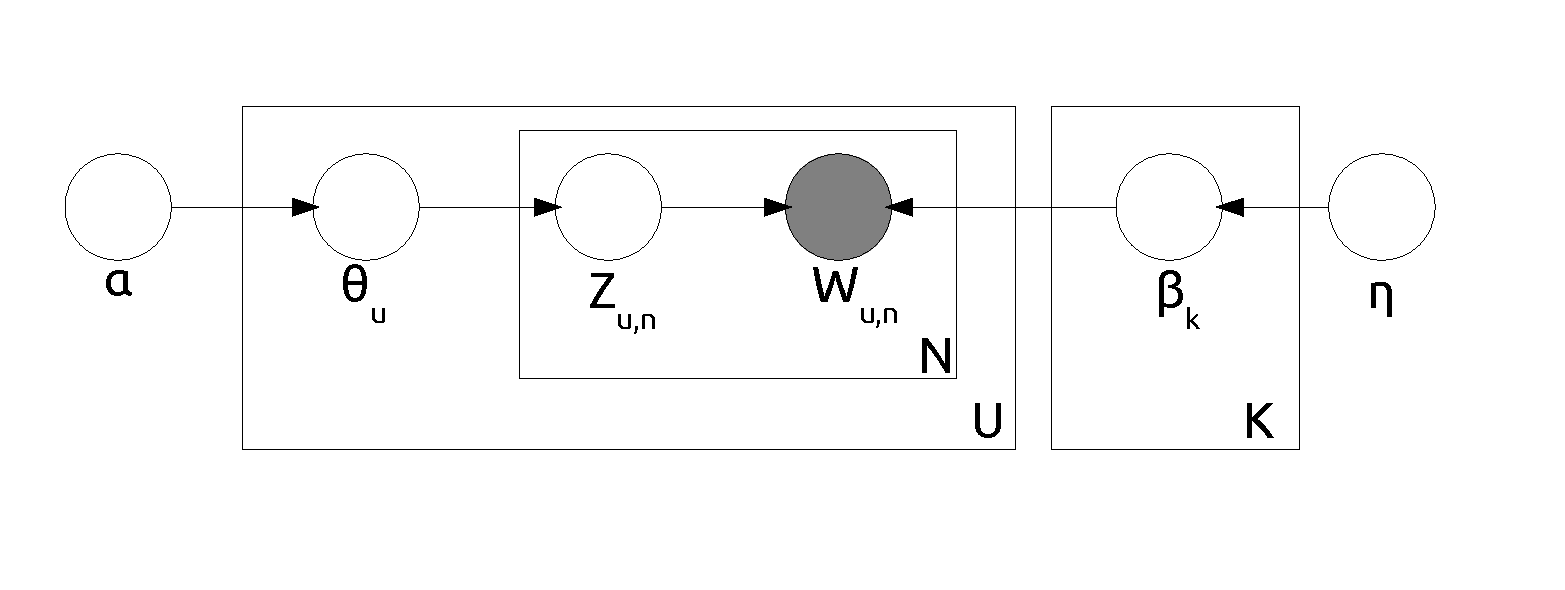
\includegraphics[width=3.0in,height=1.2in]{LDA.pdf}
%\vspace{-4em}
\caption{Plate illustration of the user-level LDA model.}
\label{fig:graph2}
\end{figure}

Formally, given a set of users $ U $ and the number of topics $ K $, a user $u$ ($ u \in U $) could be represented by a multinomial distribution $ \theta_{u} $ over topics with a Dirichlet prior parameterized by $ \alpha $. 
A topic $ k $ ($ k \in K $) is represented by a multinomial distribution $ \beta_{k} $ with another Dirichlet prior parameterized by $ \eta $. 
The generative process works as follows:
\begin{itemize*}
\item For each user $ u $, draw $ \theta_{u} \sim Dir \left(  \alpha \right) $.
\item For each word $ w_{u,n} $ in a user document, $ n \in \left\lbrace 1, \cdots, N \right\rbrace $ :
\begin{itemize*}
\item draw a topic $ z_{u,n} \sim Multinomial \left( \theta_{u}  \right) $;
\item draw a word $ w_{u,n} $ from multinomial probability\\ $  p \left( w_{u,n} \vert z_{u,n}, \beta_{k}  \right) $ conditioned on the topic $ z_{u,n} $.
\end{itemize*}
\end{itemize*}
The parameters $ \theta_{u} $ and each $ \beta_{k} $ can be estimated by Gibbs sampling or variational inference.
We use variational inference-based topic model package Gensim \cite{rehurek_lrec}.

\subsubsection{Sentiment Analysis for Tweets}
\label{sentiment}
Users often express opinions towards their topics of interest by publishing topic-related tweets. 
In order to explore the opinions of users, we need to understand sentiment embedded in each tweet.
Sentiment analysis mainly use machine learning or rule-based approaches. 
Machine learning approaches often needs labelled data for the training process, which is often impossible for Twitter because of the large volume of tweets and its dynamic language characteristics. Therefore we adopt rule-based approaches, which could adapt to Twitter with good flexibility by changing its particular characteristics into rules \cite{Thelwall:2010SSS,Hu:2013www}.

The rule-based SentiStrength package has been built especially to cope with sentiment analysis in short informal text of social media \cite{Thelwall:2010SSS}.
It combines lexicon-based approaches with sophisticated linguistic rules adapted to social media, which is suitable for analyzing sentiment of tweets in our research settings.
SentiStrength assigns two values to each tweet standing for sentiment strengths: a positive and a negative sentiment measurement, both ranging from 1 to 5 on absolute integer scales, with 1 denoting neutral sentiment and 5 denoting highest sentiment strength.
Sentiment assigned by SentiStrength is not a simple binary value but a fine-grained strength, which can catch fine opinion distributions of a user's subjective model. 
For the convenience of distribution calculation, we map the output of SentiStrength to single-scaled sentiment valence space $ \left[ 0, 8 \right] $ as follows:
\begin{equation}
\label{opinionmap}
o= \left\{ 
\begin{array}{lll}
{p+3} & if \vert p \vert > \vert n \vert \\
{n+5} & \text{if } \vert n \vert > \vert p \vert \\
{4}  & \text{if } \vert p \vert = \vert n \vert
\end{array}
\right.
\end{equation}
Where $ p $ denotes the positive setiment strength and $ n $ denotes negative sentment strength.
In the sentiment valence space, value 4 indicates neutral sentiment, while values above 4 indicate positive sentiment and values below 4 indicate negative sentiment. In this way, we can aggregate all sentiments towards a topic as a opinion distribution over sentiment valence space.

\subsubsection{Concrete Subjective Model}
\label{concrete}
With statistical topic analysis and sentiment analysis described above, we can concrete subjective model in a local network settings now. 
For user set $ U $ of a local network, we denote tweet set published by a user $ u $ as $ C_{u}=\left\lbrace c_{i} \vert i \in \left[ 1, \cdots, N \right]  \right\rbrace$. Each $ C_{u} $ is concatenated to a single document $ d_{u} $ to construct Local Topic Space $ T=\left\lbrace t_{i} \vert i=1, \cdots, K \right\rbrace $.
In the Local Topic Space $ T $, a topic model is built with parameter $ \theta $\ representing the distribution of each user over topics he tweets about, and
parameter $ \beta $ represents the distribution of each topic over the vocabulary of all tweets. SentiStrength is applied to each tweet $ c $ in collection $ C_{u} $ and outputs sentiment strength $ s_{c} $ for tweet $ c $. 
We build the subjective model of user $ u $ as follows:
\begin{itemize*}
\item Firstly, for user $ u $, the corresponding component $ \theta_{u} $ is his topic distribution in the Local Topic Space $ T $. $ p\left( z_{u} \vert \theta_{u} \right)  $ could be regarded as the weight of subjective model $ w_{u} \left( t_{i} \right)  $, and topics he tweets about are $ Z_{u}= \left\lbrace z_{u} \vert p\left( z_{u} \vert \theta_{u} \right)>0 \right\rbrace $.
\item Secondly, the topic model of Local Topic Space $ T $ is applied to each tweet $ c $ to find topics of $ c $, which are $ Z_{c} =\left\lbrace z_{c} \vert p\left( z_{c} \vert \theta, \beta, Z_{u} \right)>0 \right\rbrace $.
\item Thirdly, the opinion distribution of user $ u $ towards topic $ t \in Z_{u} $ could be calculated as:
\begin{equation}
\label{opinionall}
d_{u,t}\left( o \right) = \left\lbrace \dfrac{N_{o}}{\sum_{o \in O} N_{o}} \vert O=\left[ 0, \cdots, 8 \right] \right\rbrace 
\end{equation}
where $ N_{o} $ is the number of times user $ u $ expresses an opinion to topic $ t $ with sentiment strength $ o $, which could be calculated as:
\begin{equation}
\label{opinion1}
N_{o}=\sum_{c \in Cu} I\left( s_{c} \right) , \text{ if } s_{c}=o \& t \in Z_{c}
\end{equation}
\begin{equation}
\label{opinion2}
I\left( s_{c} \right)=\left\{
\begin{array}{ll}
{1} & \text{if } s_{c}=o \& t \in Z_{c}\\
{0} & \text{else}
\end{array}
\right.
\end{equation}

where $ s_{c} $ denotes the sentiment strength of tweet $ c $, and for simplicity, we assume the sentiment of tweet $ c $ is related to every topic it talks about in $ Z_{c} $.

\end{itemize*}

Totally, we build subjective model $ P\left( u \right) $ for user $ u $ as:
\begin{equation}
\label{subuser}
P\left( u \right)= \left\lbrace \left( t, p\left( z_{u} \vert \theta_{u} \right), d_{u,t}\left( o \right) \right)  \vert t \in Z_{u}, o \in O  \right\rbrace  
\end{equation}
and accordingly subjective model $ P\left( c \right) $ for tweet $ c $ as:
\begin{equation}
\label{subtweet}
P\left( c \right)= \left\lbrace \left( t, p\left( z_{c} \vert \theta, \beta \right), d_{c,t}\left( o \right) \right)  \vert t \in Z_{c}, o \in O  \right\rbrace  
\end{equation}

\subsection{Retweeting Analysis With Subjective Model}
\label{formulation}
To understand the underlying reasons why a user retweet a message, we try to simulate the subjective decision-making procedure by investigating the relationship among subjective models of a tweet, its publisher and followers. 
We assume that a user retweet a message because the user not only finds its topics interesting but also shares similar opinions towards these topics. In other words, if the subjective models of a tweet and a user are similar enough, the user will have a very high probability to retweet the tweet. 
We call this phenomenon as ``resonanace'', and assume resonanace between tweet and users will elicit retweeting behavior.
With the subjective models built for users and tweets, we can define a similarity measurement to quantify the resonanace among them.

Formally, for a tweet $ c $, the corresponding publisher $ p $, and a list of followers $ F= \left\lbrace f_{i} \vert i=1, \cdots, N \right\rbrace  $, for each $ f_{i} \in F $, we can define a quadruple $ < f_{i}, p, c, r_{fpc} >  $ as Section~\ref{statement}.
We firstly build subjective model $ P\left( u \right)  $ for each user $ u \in F \bigcup p $ and $ P\left( c \right)  $ for tweet $ c $, then define the similarity measurement as follows:
\begin{equation}
Sim\left( c,f_{i} \right) = similar\left( P\left( c \right), P\left( f_{i} \right) \right)
\end{equation}
according to Equation~\ref{subuser},\ref{subtweet}:
\begin{equation}
\label{tweetfollower}
\begin{split}
Sim\left( c,f_{i} \right) = \lambda \ast Dist\left( p\left( z_{c} \vert \theta, \beta \right), p\left( z_{f_{i}} \vert \theta_{f_{i}} \right) \right) \\
+\left(1-\lambda \right) \ast \left( \sum_{t \in T} Dist \left( d_{c,t}, d_{f_{i}, t} \right)  \right)
\end{split}
\end{equation}
where 
\begin{itemize*}
\item $ \lambda $ is the coefficient used to control the proportions of topic similarity and opinion similarity in the holistic subjective similarity. We initiate it by setting $ \lambda =0.5 $, and model different factors by adjusting its value in the experiment. 
\item $ Dist $ is the similarity measurement between two distribution, we choose \emph{Cosine Similarity } in our research among different measurements.
\end{itemize*}
We also assume that a user might retweet another user because of their subjective resonanace. Accordingly we define similarity between publisher $ p $ and follower $ f_{i} $ as :
\begin{equation}
\label{pubfollower}
\begin{split}
Sim\left( p,f_{i} \right) = \lambda \ast Dist\left( p\left( z_{p} \vert \theta_{p} \right), p\left( z_{f_{i}} \vert \theta_{f_{i}} \right) \right) \\
+\left(1-\lambda \right) \ast \left( \sum_{t \in T} Dist \left( d_{p,t}, d_{f_{i}, t} \right)  \right)
\end{split}
\end{equation}

\section{Experiment}
\label{experiment}
In this section, we investigate whether subjective model can help retweet analysis on an off-the-shelf dataset. 

\subsection{Dataset}
Because there is no publicly annotated dataset for retweeting analysis, We adopt an off-the-shelf Twitter dataset of previous work\cite{Luo:2013RMF}, which was created using Twitter API\footnote{\url{https://dev.twitter.com/}} with posting time from September 14th, 2012 to October 1st, 2012.
To form the dataset, randomly selected English tweets which had been retweeted at least once were used as test tweets, then each tweet was chosen as starting point to collect data of its publisher and followers.
Summary statistics of the dataset are listed in Table~\ref{datasetstat}.
\begin{table}
\centering
\caption{Retweet Dataset Statistics}
\label{datasetstat}
\begin{tabular}{|c|c|}
\hline
Total tweets which have been retweeted & 500 \\
Average number of followers per tweet & 89 \\
Total retweeters & 5214 \\
Total non-retweeters & 40317  \\
\hline
\end{tabular}
\end{table}
In the dataset, there are 500 test tweets and corresponding publishers, 4,5531 followers, 6,277,736 published tweets, and 5214 retweeters who retweet at least one test tweet. 
Their relations are illustrated in Figure~\ref{fig:graph3}.
\begin{figure}[htb]
%\setlength{\belowcaptionskip}{-0.2cm} 
\centering%
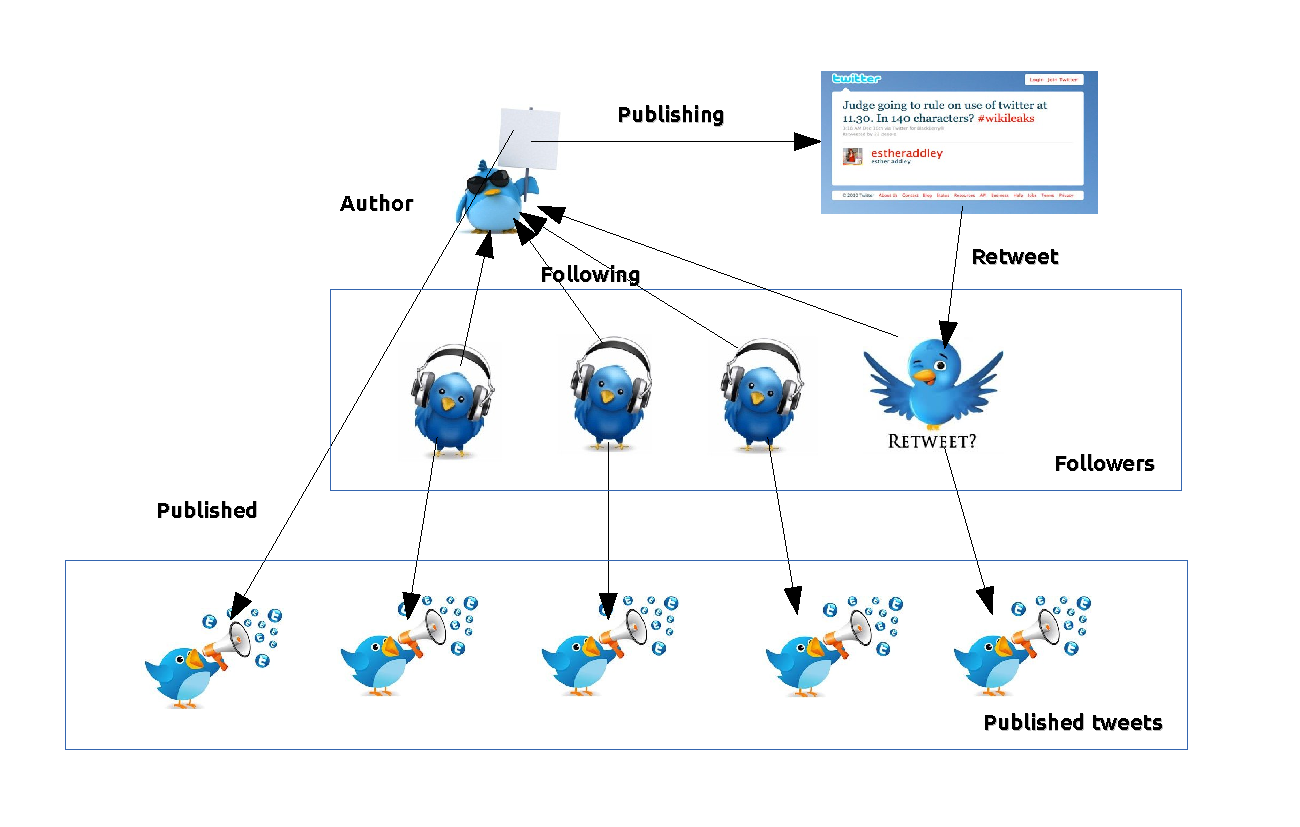
\includegraphics[width=3.5in,height=2.1in]{dataset.pdf}
%\vspace{-4em}
\caption{Illustration of dataset structure.}
\label{fig:graph3}
\end{figure}
There is a local network structure for each test tweet as figure shows, consisting of its publisher and followers.

\subsection{Impact on Retweeting}
\label{influence}
In Section~\ref{formulation},  we model retweeting behavior with subjective model in the form of similarity measurements~\ref{tweetfollower},\ref{pubfollower}.
By setting different value to $ \lambda $, the measurements can be transformed into different versions to model different factors that might influence user's retweeting behavior, which are:
\begin{itemize*}
\item \textbf{TTF}: \textbf{T}opic similarity between \textbf{T}weet and each \textbf{F}ollower $ \left( \lambda =1  \text{ in measurement~\ref{tweetfollower}} \right) $ 
\item \textbf{OTF}: \textbf{O}pinion similarity between \textbf{T}weet and each \textbf{F}ollower $ \left( \lambda =0 \text{ in measurement~\ref{tweetfollower}} \right) $
\item \textbf{STF}: \textbf{S}ubjective similarity between \textbf{T}weet and each \textbf{F}ollower $ \left( \lambda \in \left( 0,1 \right)   \text{ in measurement~\ref{tweetfollower}} \right) $ 
\item \textbf{TPF}: \textbf{T}opic similarity between \textbf{P}ublisher and each \textbf{F}ollower $ \left( \lambda =1  \text{ in measurement~\ref{pubfollower}}  \right) $ 
\item \textbf{OPF}: \textbf{O}pinion similarity between \textbf{P}ublisher and each \textbf{F}ollower $ \left( \lambda =0 \text{ in measurement~\ref{pubfollower}} \right) $
\item \textbf{SPF}: \textbf{S}ubjective similarity between \textbf{P}ublisher and each \textbf{F}ollower $ \left( \lambda \in \left( 0,1 \right)   \text{ in measurement~\ref{pubfollower}} \right) $
\end{itemize*}
The six similarity measurements could be grouped into two aspects. 
One is consisted of TTF, OTF and STF, which is direct and explicit by modelling the tweet and its followers;
the other is consisted of TPF, OPF and SPF, which is indirect and implicit by modelling the tweet publisher and followers.
The two aspects reflect properly the local information diffusion structure of Twitter at micro-level as illustrated in Figure~\ref{fig:graph3}.

To analyze the impact of different factors on retweeting, we compare six average similarity scores between 5214 retweeters and 5214 randomly selected followers who do not retweet any test tweet. The values of $ \lambda $ for STF and SPF are tuned to produce the largest difference between retweeters and unretweeters, which are $ \lambda =0.5 $ on our dataset. Figure~\ref{fig:graph6} shows the result.
\begin{figure}[htb]
%\setlength{\belowcaptionskip}{-0.2cm} 
\centering
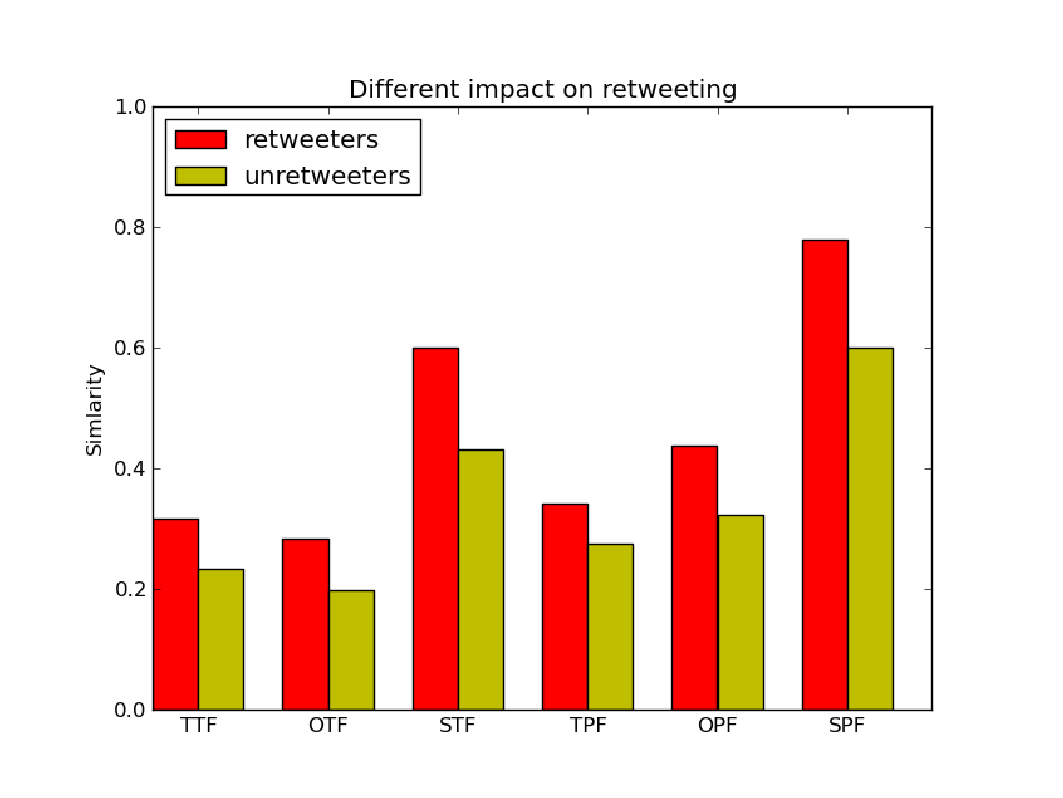
\includegraphics[width=3.8in,height=2.2in]{component.pdf}
\vspace{-2em}
\caption{Impact of different factors on retweeting.}
\label{fig:graph6}
\end{figure}
As the figure illustrated, the similarities scores of retweeters are obviously higher than other followers for all six factors. Specifically: 
\begin{itemize*}
\item TTF score shows that a tweet is more likely to be retweeted by followers who find topics it talks about interesting to them, which is consistent with other studies\cite{conf/icwsm/MacskassyM11, conf/wsdm/FengW13};
\item OTF score shows that opinions in a tweet is an important indicator to be retweeted by by followers who hold similar opinions, although other studies\cite{conf/icwsm/PfitznerGS12,2011:NaveedGKC} have shown that sentiment in tweet have impact on retweeting, they haven't consider the opinions of followers and opinion similarity betweet tweet and its followers;
\item STF score shows the subjective similarity is the most distinguishable feature among the six factors with the largest difference between retweeters and other followers, which proves the importance of subjective model;
\item TPF score gives another perspective for retweeting analysis from the topic similarity between publisher and followers, indicating that followers are more likely to retweet publisher with similar interests , which verifies the homophily principle of retweeting relation;
\item OPF score indicates that similar opinions for common topics also influence followers' decision of retweeting anothor user, which proves opinion homophily of retweeting relation.
\item SPF score is interesting in that it implies that subjective similarity between publisher and follower might cause retweeting, and we call this phenomenon ``tight homophily'' of retweeting relation because it requires both topic homophily and opinion homophily.
\end{itemize*} 

\subsection{Performance of Retweeting Prediction}
\label{performance}
The main purpose of retweeting analysis is to help users find interesting information from the overwhelming information streams. 
Retweeting is an important signal of interestingness because users are prone to broadcast their favorite messages to their followers. 
Thus, the performance of retweeting prediction is a suitable evaluation for the utility of subjective model in retweeting analysis problem.
In our experiment, we evaluate the subjective model in supervised machine learning framework.

As Section~\ref{statement} introduced, the retweeting analysis problem could be formulated as a quadruple $< f, p, c, r_{fpc} > $.
For retweeting prediction, we need to estimate the label $ r_{fpc} $ when $ c, p, \text{and } f $ are known. 
There are 5,214 retweeters in our dataset who retweet at least one test tweet, so we extract 5214 quadruples as positive instances with their label $ r_{fpc}=1 $.
For the other 40,317 followers who do not retweet any test tweet, we also extract quadruples to as negative instances with label $ r_{fpc}=0 $.
To avoid unbalance bias of training data, we randomly sample 5,214 negative instances into the final dataset.

\subsubsection{Comparison With Other User Models}
\label{comparison}
Firstly the comparison between our model with other user models (TF-IDF model \cite{Luo:2013RMF}, entity-based model and hashtag-based model \cite{Abel:2011AUM}) in retweeting prediction is investigated.
As defined in Section~\ref{influence}, the six versions derived from our model are used for comparison, because they model different factors that influence retweeting baehavior.
For the comparing models, cosine similarities are calculated between tweets and their followers.
We use the logistic regression classifier of Scikit-learn machine learning package \cite{scikit-learn} for training, with 5-fold cross-validation on our balance dataset. Accuracy is our evaluation metric.
Performances of our model and all other models are shown in Figure~\ref{fig:graph7}.
\begin{figure}[htb]
%\setlength{\belowcaptionskip}{-0.2cm} 
\centering
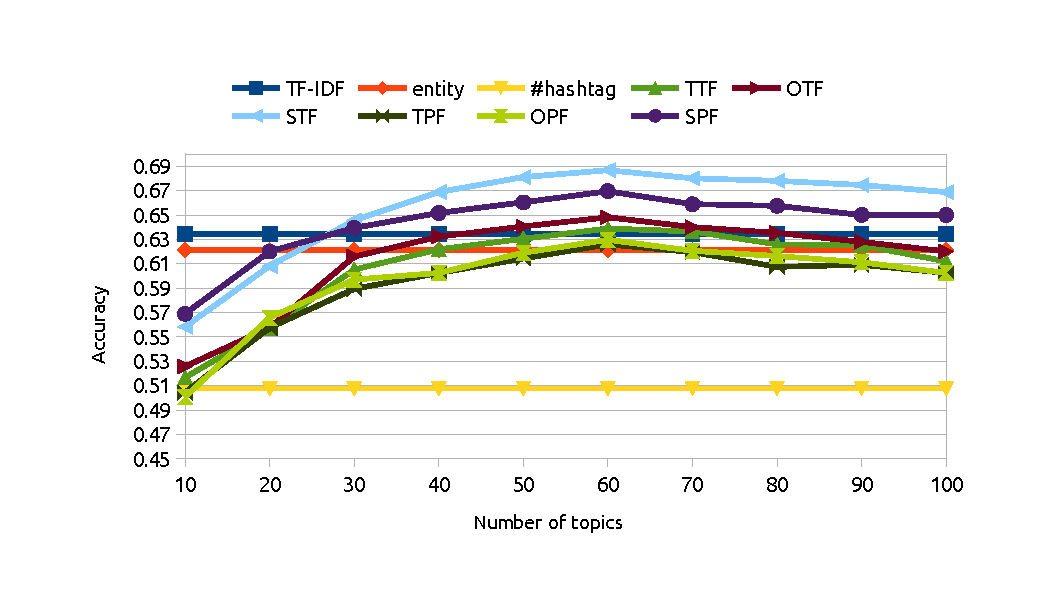
\includegraphics[width=3.5in,height=2.2in]{comparison.pdf}
%\vspace{-4em}
\caption{Comparison of different models.}
\label{fig:graph7}
\end{figure}
Figure~\ref{fig:graph7} shows that the impact of topic number of LDA on the predicting accuracy, our model arrives its peak when the number is set to 60, so we fix the topic number as 60 in all our experiment.

As Figure~\ref{fig:graph7} illustrates, the best accuracy of 68.67\% is achieved by the STF (Subjective similarity between Tweet and Followers) model .
The accuracies of TF-IDF model and entity-based model are 63.45\% and 62.12\%, which are very close to TTF (Topic similarity between Tweet and Followers, 63.88\%) model and OPF (Opinion similarity between Publisher and Followers, 62.96\%) model.
While for hashtag-based model, its accuracy is  50.76\% , which is only a little better than random selection (50\%) but not significant. The reason might lie in a very low usage of hashtagin our data. 
The accuracies of the other three model are OTF (Opinion similarity between Tweet and Followers) model 64.80\%, TPF (Topic similarity between Publisher and Followers) model 62.58\% and SPF (Subjective similarity between Publisher and Followers) model 66.95\%.
The results show that subjective model can better help understand retweeting behavior than the other user models.

\subsubsection{Retweeting Classification Evaluation}
\label{classifiction}
In this section, we feed the six versions of our model as features into a retweeting classification framework to verify the effectiveness of subjective model. 
We compare the performance of our model with method of Luo \emph{et al.}~\cite{Luo:2013RMF} which uses four feature families: Retweet History(follower who retweeted a user before is likely to retweet the user again), Follower Status(for a follower, the number of tweets, followers, friends, being listed he has and whether he is verified), Follower Active Time(the time users interact with others) and Follower Interests(common interests between tweet and followers, they use ``bag-of-words'' to model the followers interests).

We use LinearSVM of Scikit-learn package to build a retweeting prediction model, leveraging two different features sets. One includes the six features derived from subjective model (marked as ``SM6''). The other is feature set from Luo \emph{et al.}~\cite{Luo:2013RMF}(marked as ``LUO''). We use the same dataset as introduced in Section~\ref{comparison} with 5-fold cross-validation, and accuracy as evaluation metric.
In addition, we set a baseline (marked as ``RB''), for which followers who have retweeted the publisher's previous tweets are predicted as retweeters of current tweet. 
The result is listed in Table~\ref{table2}.
\begin{table}
\centering
\caption{Prediction Accuracy of Different Models. Significant improvement over baseline with star($ \ast $) and LUO' model with dagger($ \ddagger $) (p$ < $0.05).}
\label{table2}
\begin{tabular}{|l|l|}
\hline
Feature Set & Accuracy(\%) \\
\hline
RB & 60.85  \\
LUO & 68.76 $ \ast  $\\
SM6 & 69.12  $ \ast $ \\
LUO($ \ominus $)+TTF & 69.20  $ \ast $ \\
LUO($ \ominus $)+TPF & 71.04  $ \ast \quad \ddagger $ \\
LUO($ \ominus $)+OTF & 71.88  $ \ast \quad \ddagger $ \\
LUO($ \ominus $)+OPF & 70.27  $ \ast $ \\
LUO($ \ominus $)+STF & 72.86  $ \ast \quad \ddagger $ \\
LUO($ \ominus $)+SPF & 72.05  $ \ast \quad \ddagger $ \\
LUO($ \ominus $)+All & 72.93  $ \ast \quad \ddagger $ \\
\hline
\end{tabular}
\end{table}
The accuracy of baseline is 60.85\%, and two prediction models(LUO and our SM6) both outperform the baseline significantly. 
But the prediction model based on our feature set shows no significant improvement over the model based on LUO feature set. 
The reason might be that our model only tries to reflect the retweeting motivation of users based on content, whereas other important factors associated with retweeting behavior are not considered, such as network context and reading habit of the user, etc. 

Since it is proved that subjective model outperforms bag-of-words model in Section~\ref{comparison}, which is used in LUO feature set, we propose that retweeting prediction performance could be improved by using features derived from subjective model. 
As denoted by ``LUO($ \ominus $)+'' in the table, the Follower Interests features of LUO are replaced with our six features one by one. 
The accuracies are all improved. It shows that our model is of great importance for retweeting prediction. 
Noticing that, the most significant improvement (LUO($ \ominus $)+STF, 72.86\% versus 68.76\%) is the subjective similarity feature between tweet and followers, which verifies our assumption that subjective resonanace between tweet and followers can be considered as the underlying reason that elicits retweeting behavior.
Besides, the improvement by adding subjective similarity features between publisher and followers (LUO($ \ominus $)+SPF, 72.05\% versus 68.76\%) is also obvious in that the resonanace between publisher and follower indicates the tight homophily between them.
Finally, the last row of table is the complete combination of two sets of features (LUO($ \ominus $)+All) by adding all six features into LUO feature set. 
The performance shows no significant improvement over adding STF feature only, in that subjective model combines both topic and opinion information, and STF is a integral feature to model both topic similarity and opinion similarity between tweet and followers, so it is redundant to add other separate parts.

\subsection{Case Study}
\label{example}
In this section we give an qualitative description about subjective model and its ability in explaining the retweet behavior with an intuitive example. 
Subjective models for one of the 500 test tweets, its publisher, and two followers (one retweet it while the other does not) are shown as Figure~\ref{fig:graph4}. 
The right part of each sub-figure illustrates topic distribution and the left part illustrates opinion distribution for each topic. 
It is the 14th topic that the tweet talks about in the local topic space.
\begin{figure*}[htb]
%\setlength{\belowcaptionskip}{-0.2cm} 
\centering%,bb=0 0 1280 960
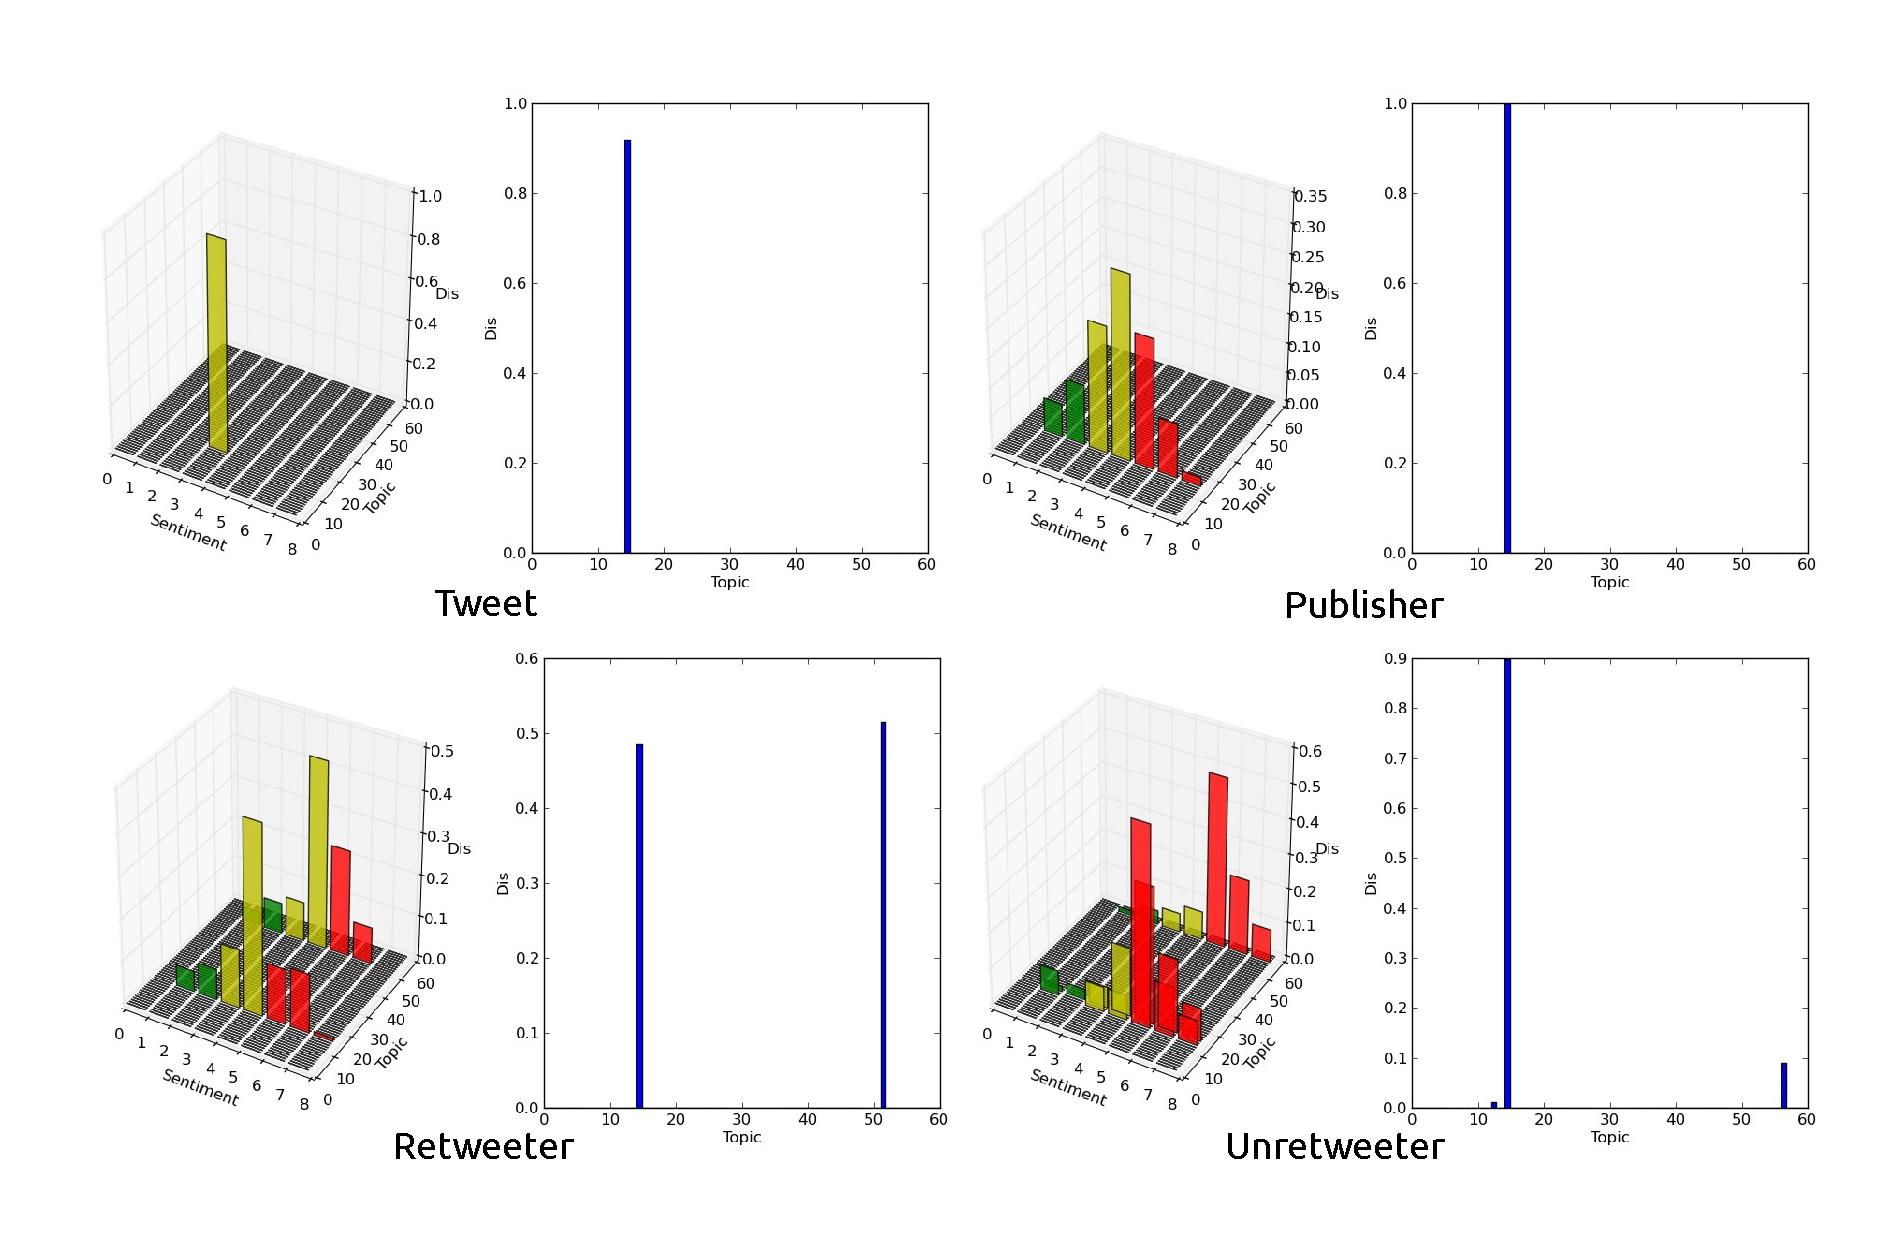
\includegraphics[width=6.5in,height=3.8in]{tweets10.pdf}
%\vspace{-4em}
\caption{Subjective model examples.}
\label{fig:graph4}
\end{figure*}
Figure~\ref{fig:graph5} shows top words of the 14th topic, the tweets of publishers and two followers in a word cloud\footnote{We use TagCrowd (\url{http://tagcrowd.com/}) to produce word cloud.}.
\begin{figure}[htb]
%\setlength{\belowcaptionskip}{-0.2cm} 
\centering
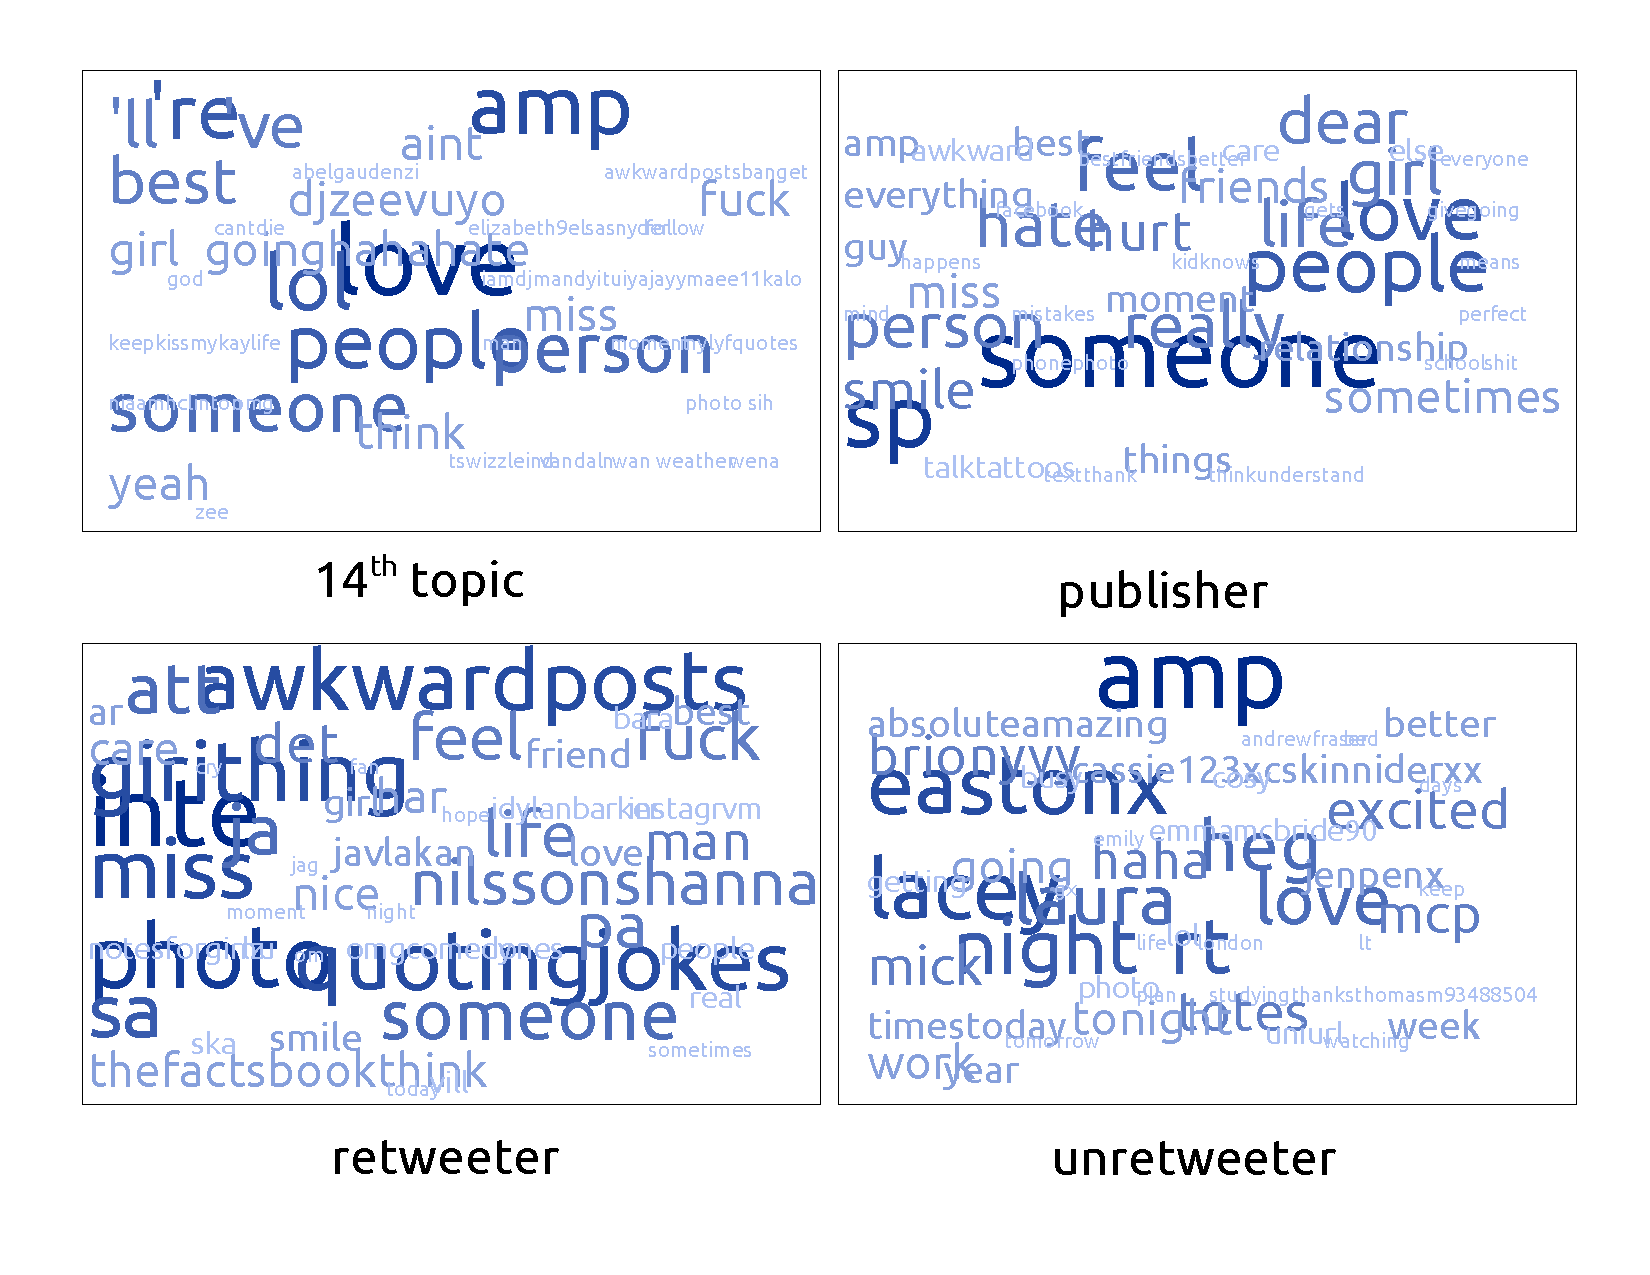
\includegraphics[width=3.5in,height=2.2in]{text_cloud.pdf}
%\vspace{-3em}
\caption{Word cloud of 14th topic, publisher and followers}
\label{fig:graph5}
\end{figure}
Content of the tweet is:\\
\textit{Tweet: ``Sometimes the right person for you was there all along. You just didn’t see it because the wrong one was blocking the sight''} \\
The topic of this tweet is about ``love between people'' and the opinion is neutral, which is in accordance with the 14th topic word cloud in Figure~\ref{fig:graph5} and subjective model of tweet in Firgure~\ref{fig:graph4}.
The publisher concentrates on ``love between people'' topic, and his opinions are mainly neutral (as Figure~\ref{fig:graph4},~\ref{fig:graph5} demonstrate).
As for two followers, the ``retweeter'', has published tweets about two topics (the 14th and 52nd topic) uniformly and his opinions towards the two topics are mainly neutral.
While the other one, the ``unretweeter'', has also talked about two topics (14th and 56th topic), but he is mainly interested in 14th topic and has positive opinion.
Although two followers have same interest (the 14th topic), their different opinions elicit their different decision, which verifies subjective model can help better understand the retweeting behavior.

\section{Conclusion}
In this paper, we propose subjective model to analyze user retweeting behavior on Twitter. We assume that retweeting should be elicited by the subjective resonanace between the tweet and its followers. 
We define subjective model formally as the combination of topic distribution and opinion distribution, and we concrete subjective model leveraging statistical topic model and sentiment analysis techniques.
We demonstrate the effectiveness of our model for retweeting analysis problem and show that subjective model is able to reach better understanding of retweeting behavior. 

Our future work mainly lie in two directions.
Firstly, subjective model is established through simple combination of topics and opinions. It is an interesting direction to establish it under the framework of generative topic-sentiment model, which has been applied in reviews and citation network.
Secondly, we will apply subjective model to other social media analysis task such as connection prediction and friend recommendation.
\bibliographystyle{abbrv}
\bibliography{resonate_tweet}
\end{document}
